\documentclass[12pt]{article}

% TEMPLATE DEFAULT PACKAGES
\usepackage{amssymb,amsmath,amsfonts,eurosym,geometry,ulem,graphicx,color,setspace,sectsty,comment,natbib,pdflscape,array,adjustbox}

% ADDED PACKAGES FOR THIS MANUSCRIPT
\usepackage{palatino,newtxmath,multirow,titlesec,threeparttable,tabu,booktabs,titlesec,threeparttable,mathtools,bm,bbm,subcaption,pdflscape,tcolorbox,mathrsfs,tikz,graphicx}
% endfloat,

\usepackage{afterpage}
\usepackage[hyphens]{url}
\usepackage[margin=1cm]{caption}

\usepackage[draft]{hyperref}
\newcommand{\tim}{$\,\times\,$}
% FIGURES & TABLES CAPTION STYLING
\captionsetup[figure]{labelfont={bf},name={Figure},labelsep=period}
\captionsetup[table]{labelfont={bf},name={Table},labelsep=period}

% SECTION TITLE SETTINGS
\titlelabel{\thetitle.\enskip}
\titleformat*{\section}{\large\bfseries}
\titleformat*{\subsection}{\normalsize\bfseries}

% COLUMN TYPES
\newcolumntype{L}[1]{>{\raggedright\let\newline\\\arraybackslash\hspace{0pt}}m{#1}}
\newcolumntype{C}{>{\centering\arraybackslash}p{5.2em}}
\newcolumntype{D}{>{\centering\arraybackslash}p{5em}}
\newcolumntype{R}[1]{>{\raggedleft\let\newline\\\arraybackslash\hspace{0pt}}m{#1}}


% MARGINS AND SPACING
\normalem
\geometry{left=1.1in,right=1.1in,top=1.0in,bottom=1.0in}
\setlength{\parskip}{2.5pt}

% SPECIAL CELL 
\newcommand{\specialcell}[2][c]{%
	\begin{tabular}[#1]{@{}l@{}}#2\end{tabular}}

% NO INDENT ON FOOTNOTES
\usepackage[hang,flushmargin]{footmisc}

\begin{document}


\begin{figure}
\centering
\caption{Average Demeaned Deaths by Temp. Before and After Winter policy goes into effect each year}
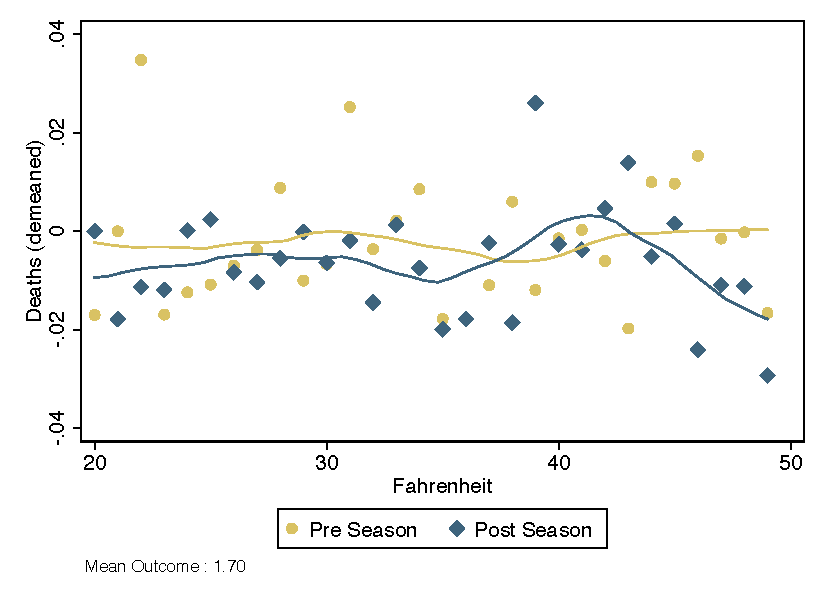
\includegraphics[scale=.8]{figures/tgrad_deaths_all.pdf}
\end{figure}


\begin{figure}
\centering
\caption{Average Demeaned Deaths by one day lag Temp. Before and After Winter policy goes into effect each year}
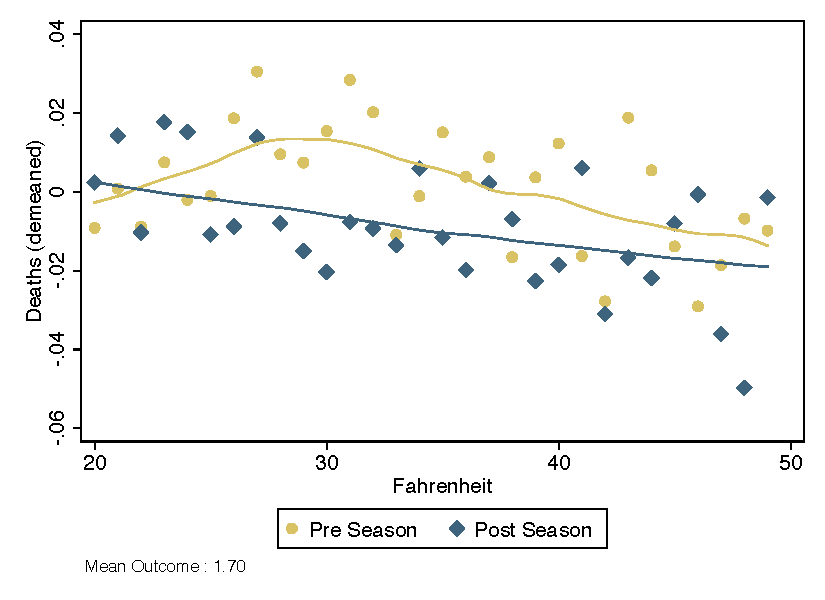
\includegraphics[scale=.8]{figures/tgrad_deaths_all_lag1.pdf}
\end{figure}


\begin{figure}
\centering
\caption{Average Demeaned Deaths by  two day lag Temp. Before and After Winter policy goes into effect each year}
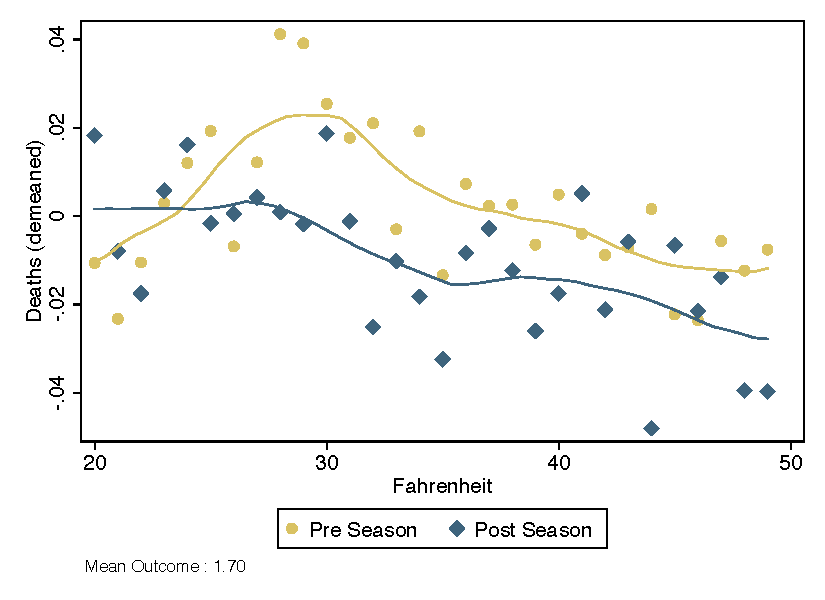
\includegraphics[scale=.8]{figures/tgrad_deaths_all_lag2.pdf}
\end{figure}



\begin{figure}
\centering
\caption{Average Demeaned Cold-Sensitive Deaths by Temp. Before and After Winter policy goes into effect each year}
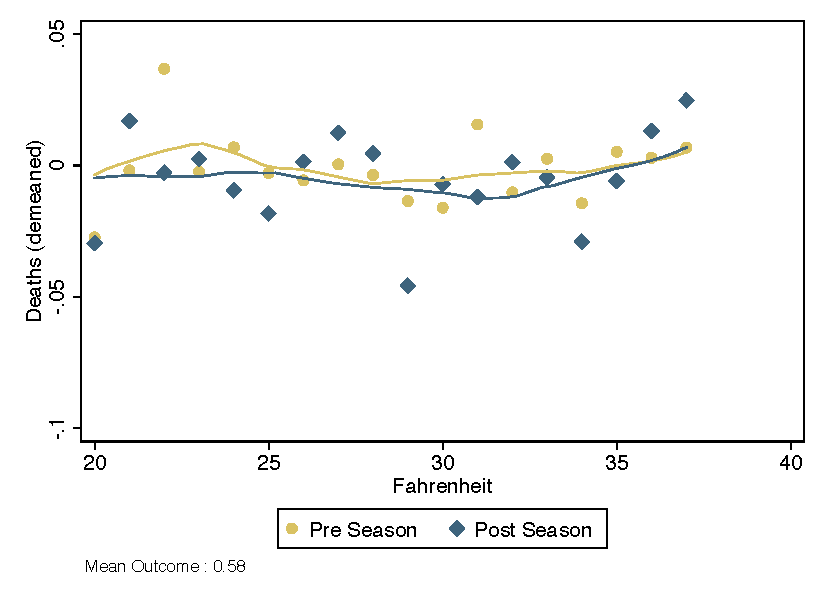
\includegraphics[scale=.8]{figures/tgrad_deaths_ewm.pdf}
\end{figure}


\begin{figure}
\centering
\caption{Average Demeaned Cold-Sensitive Deaths by one day lag Temp. Before and After Winter policy goes into effect each year}
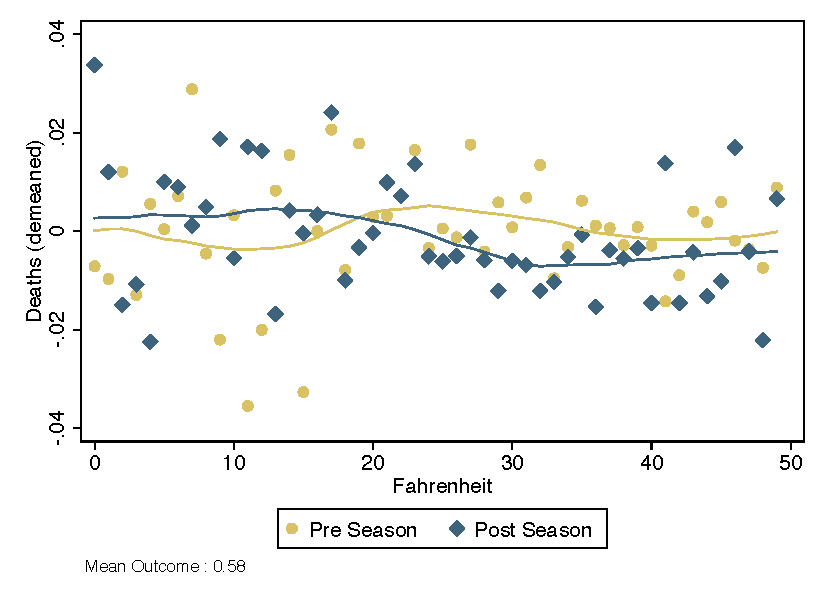
\includegraphics[scale=.8]{figures/tgrad_deaths_ewm_lag1.pdf}
\end{figure}


\begin{figure}
\centering
\caption{Average Demeaned Cold-Sensitive Deaths by  two day lag Temp. Before and After Winter policy goes into effect each year}
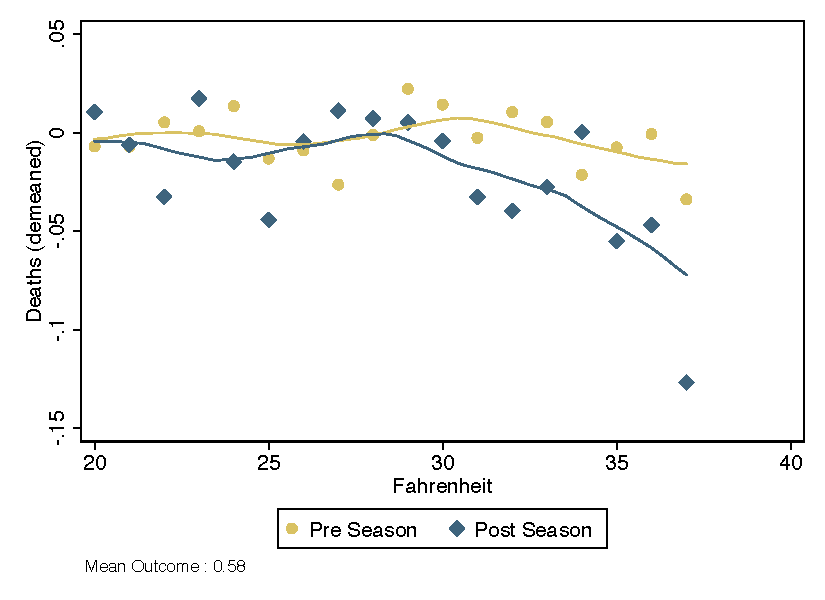
\includegraphics[scale=.8]{figures/tgrad_deaths_ewm_lag2.pdf}
\end{figure}




% \begin{itemize}
% \item Plot event-studies before and after seasonal start and end dates (before and after policies are in place)
%     \begin{itemize}
%         \item conduct at state-level (look at cold and warm deaths separately)
%         \item demean by calendar-day and state-year
%     \end{itemize}
% \end{itemize}



\end{document}


